% Written By Enoch Yu
% Downloaded from archive.enochyu.com

\documentclass{article}

\usepackage{amsmath}
\usepackage{amsthm}
\usepackage{amssymb}
\usepackage{gensymb}
\usepackage[margin=1in]{geometry}

\usepackage{tikz}
\usetikzlibrary{calc, angles, quotes}
\usepackage{tkz-euclide}
\usepackage{graphicx}
\usepackage{float}
\usepackage[font=small,labelfont=bf]{caption}

\usepackage[normalem]{ulem}
\usepackage{hyperref}
\hypersetup{
    colorlinks=true,
    linkcolor=blue,
    filecolor=magenta,
    urlcolor=cyan,
    pdftitle={Problem Set 3},
    pdfpagemode=FullScreen,
}

\usepackage{parskip}
\usepackage{fancyhdr}
\pagestyle{fancy}
\fancyhead[R]{Enoch Yu}
\pagenumbering{gobble}

\usepackage{enumitem}
\newtheorem{theorem}{Theorem}[section]
\newtheorem{lemma}[theorem]{Lemma}
\newtheorem{sublemma}{Lemma}[section]
\newtheorem{proposition}{Proposition}
\newtheorem{corollary}{Corollary}[theorem]
\newenvironment{solution}{\begin{trivlist}\item[]
{\bf Solution}}{\qed \end{trivlist}}


\title{Problem Set 3}
\author{Enoch Yu}
\date{May 2025}

\begin{document}

\section*{Problem}
In $\triangle{ABC}$, $D$ and $E$ are points on $AB$
and $AC$ respectively. If $AB=33$, $AC=21$, $BC=m$
and $AD = DE = ED = n$ where $m$, $n$ are integers,
find the value of $m$.

\begin{solution}

\textbf{Key Word} Law of Cosines
\begin{center}
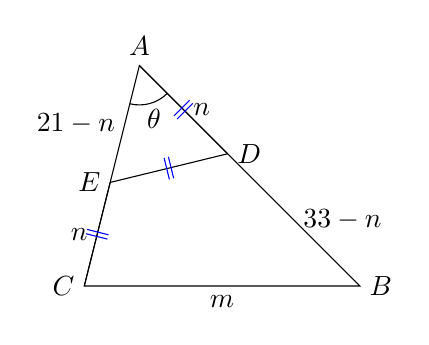
\begin{tikzpicture}[scale=0.7]
    \coordinate (A) at (1, 4);
    \coordinate (B) at (5, 0);
    \coordinate (C) at (0, 0);
    \coordinate (D) at ($(A)!0.4!(B)$);
    \coordinate (E) at ($(A)!0.53!(C)$);

    \draw (A) -- (B) -- (C) -- cycle;
    \draw (A) -- (D);
    \draw (E) -- (D);
    \draw (E) -- (C);

    \node[above] at (A) {$A$};
    \node[left] at (C) {$C$};
    \node[right] at (B) {$B$};
    \node[left] at (E) {$E$};
    \node[right] at (D) {$D$};
    \node[right] at ($(D)!0.5!(B)$) {$33-n$};
    \node[left] at ($(A)!0.5!(E)$) {$21-n$};
    \node[left] at ($(E)!0.5!(C)$) {$n$};
    \node[below] at ($(C)!0.5!(B)$) {$m$};
    \node[right] at ($(A)!0.5!(D)$) {$n$};

    \tkzMarkSegment[color=blue, pos=.5, mark=||](A,D);
    \tkzMarkSegment[color=blue, pos=.5, mark=||](D,E);
    \tkzMarkSegment[color=blue, pos=.5, mark=||](E,C);

    \draw pic[draw=black, radius=0.1cm, "$\theta$",
        angle eccentricity=1.4] {angle=E--A--D};
\end{tikzpicture}
\end{center}
Using angle $\theta$ and the Law of Cosines, two
equations may be derived.
\begin{align*}
    \cos\theta
    &= \frac{ n^2 + (21 - n)^2 - n^2 }
        { 2 \cdot n \cdot (21 - n) } \\
    &= \frac{ 21^2 + 33^2- m^2 }{ 2 \cdot 21 \cdot 33 }
\end{align*}
Therefore,
\[
\frac{21 - n}{n} =
\frac{21^2 + 33^2 - m^2}{2 \cdot 21 \cdot 33}.
\]
By rearranging the equation, the relationship between
$n$ and $m$ could be found since $n$ and $m$ are
positive integers.
\begin{align*}
    21 \cdot 33 (21 - n) &= n (21^2 + 33^2 - m^2) \\
    21^2 \cdot 33 - 21 \cdot 33n &=
        n (21^2 + 33^2 - m^2) \\
    n (21^2 + 33^2 + 21 \cdot 33 - m^2) &= 21^2 \cdot 33
\end{align*}
Using the property of triangle, the range for
$n$ and $m$ could be narrowed.
\[
\begin{array}{cccc}
   \textbf{Case I for $m$} & & & \textbf{Case II for $m$} \\
    m < 33 \leadsto m + 21 > 33 & & & m
    > 33 \leadsto 21 + 33 > m \\
    \therefore 12 < m < 33 & & & \therefore 33 < m < 54
\end{array}
\]
In another words, the range for $m$ is $12 < m < 54$
because $m$ could be 33. Inferring to the diagram,
it is likely that the range for $m$ is $12 < m < 33$.
\[
\begin{array}{cccc}
   \textbf{Case I for $n$} & & & \textbf{Case II for $n$} \\
    n < 21 - n \leadsto 2n > 21 - n & & &
    n > 21 - n \leadsto 21 - n + n > n \\
    \therefore 7 < n < \frac{21}{2} & & &
    \therefore \frac{21}{2} < n < 21
\end{array}
\]
In another words, the range for $n$ is $7 < n < 21$
because $n$ is an integer.

Before substituting every value in
$n (21^2 + 33^2 + 21 \cdot 33 - m^2) = 21^2 \cdot 33$,
it is evident that $n$ must include $3$, $7$, or $11$.
The only possible values for $n$ is 9 and 11. However,
$9$ leads to non-integer value of $m$. Thus, $n=11$ and
$\boxed{m=30}$.
\end{solution}

\newpage
\section*{Problem}
In $\triangle{ABC}$, $AB = 4$ and $AC = 6$. The two
tangents to the circumcircle of $\triangle{ABC}$ at
$B$ and $C$ intersect at $D$. If $A$ and $D$ are equidistant
from the line $BC$, find the length of $BC$.

\textbf{Solution I: The Typical Method}

\textbf{Key Words} Law of Cosines, Triangle Area Formula
\begin{center}
    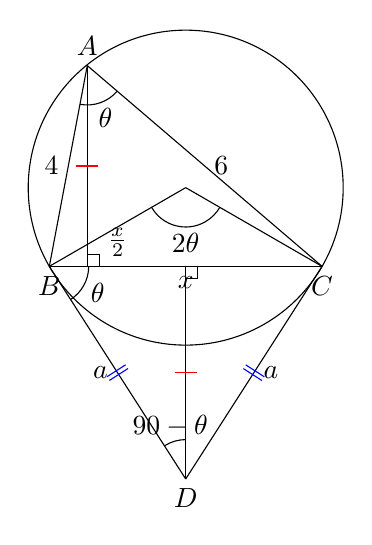
\begin{tikzpicture}

    \coordinate (A) at (-1.25, 1.55);
    \coordinate (B) at (-1.732, -1);
    \coordinate (C) at (1.732, -1);
    \coordinate (D) at (0, -3.7);
    \coordinate (E) at ($(B)!0.5!(C)$);
    \coordinate (F) at (-1.25,-1);
    \coordinate (O) at (0,0);

    \draw (-1.25, -0.85) -- (-1.10, -0.85) -- (-1.10, -1);
    \draw (0, -1.15) -- (0.15, -1.15) -- (0.15, -1);
    
    \draw[fill=none] (0,0) circle (2.0);
    \draw (B) -- (D);
    \draw (C) -- (D);
    \draw (A) -- (F);
    \draw (D) -- (E);
    \draw (B) -- (O);
    \draw (C) -- (O);
    
    \draw (A) -- (B);
    \draw (B) -- (C);
    \draw (C) -- (A);

    \node[left, above] at (A) {$A$};
    \node[left, below] at (B) {$B$};
    \node[right, below] at (C) {$C$};
    \node[below] at (D) {$D$};
    \node[left] at ($(A)!0.5!(B)$) {$4$};
    \node[right] at ($(A)!0.5!(C)$) {$6$};
    \node[below] at ($(B)!0.5!(C)$) {$x$};
    \node[above] at ($(B)!0.5!(E)$) {$\frac{x}{2}$};
    \node[left] at ($(B)!0.5!(D)$) {$a$};
    \node[right] at ($(D)!0.5!(C)$) {$a$};

    \tkzMarkSegment[color=blue, pos=.5, mark=||](B, D);
    \tkzMarkSegment[color=blue, pos=.5, mark=||](D, C);
    \tkzMarkSegment[color=red, pos=.5, mark=|](A, F);
    \tkzMarkSegment[color=red, pos=.5, mark=|](D, E);
    
    \draw pic[draw=black, radius=0.05cm, "$\theta$",
    angle eccentricity=1.4] {angle=B--A--C};
    \draw pic[draw=black, radius=0.1cm, "$2\theta$",
    angle eccentricity=1.4] {angle=B--O--C};
    \draw pic[draw=black, radius=0.1cm, "$\theta$",
    angle eccentricity=1.4] {angle=D--B--E};
    \draw pic[draw=black, radius=0.1cm, "$90-\theta$",
    angle eccentricity=1.4] {angle=E--D--B};
    \end{tikzpicture}
\end{center}
The diagram suggests that
\[
\cos\theta = \frac{x}{2a}
= \frac{4^2 + 6^2 - x^2}{2 \cdot 4 \cdot 6}.
\]
Moreover, using the fact that
$\triangle{ABC} = \triangle{BCD}$, a new equation
could be written.
\[
\frac{1}{2} \cdot 4 \cdot 6 \cdot \sin\theta
= \frac{1}{2} a^2 \sin(180 - 2\theta).
\]
Using trigonometric identities, the following
expressions are true.
\begin{align*}
    \frac{1}{2} \cdot 4 \cdot 6 \cdot \sin\theta
    &= \frac{1}{2} a^2 \sin(180 - 2\theta) \\
    \frac{1}{2} \cdot 4 \cdot 6 \cdot \sin\theta
    &= \frac{1}{2} a^2 \sin2\theta \\
    4 \cdot 6 \cdot \sin\theta
    &= a^2 \cdot 2 \sin\theta \cos\theta \\
    12 &= a^2 \cdot \cos\theta
    \text{ ($\because 0^{\circ} < \theta < 90^{\circ}$)}
\end{align*}
In another words,
\[
\cos\theta = \frac{x}{2a}
= \frac{4^2 + 6^2 - x^2}{2 \cdot 4 \cdot 6}
= \frac{12}{a^2}.
\]
Because $\frac{x}{2a} = \frac{12}{a^2}$, $ax = 24$.
From $\frac{4^2 + 6^2 - x^2}{2 \cdot 4 \cdot 6}
= \frac{52 - x^2}{48} = \frac{12}{a^2}$,
$52a^2 - a^2 x^2 = 12 \cdot 48$. $a = \frac{24}{x}$
could be substituted.
\begin{align*}
    52 \cdot \frac{24^2}{x^2} - \frac{24^2}{x^2}
    \cdot x^2 &= 12 \cdot 48 \\
    52 \cdot 24^2 - 24^2 \cdot x^2 &= 12 \cdot 48x^2 \\
    (12 \cdot 48 + 24^2) x^2 &= 52 \cdot 24^2 \\
    2x^2 &= 52 \\
    x &= \boxed{\sqrt{26}}
\end{align*}
\newpage
\textbf{Solution II: The Smart Way}

\textbf{Key Properties}

\begin{tikzpicture}[scale=1.4]
    \coordinate (A) at (-0.3, 0.95);
    \coordinate (B) at (-0.5, -0.866);
    \coordinate (C) at (0.85, -0.54);
    \coordinate (D) at (2.15, 1.5);
    \coordinate (E) at (0.25,-1.5);
    \coordinate (O) at (0,0);
    
    \draw[fill=none] (0,0) circle (1.0);
    
    \draw (A) -- (B) -- (C) -- cycle;
    \draw (O) -- (C);
    \draw (D) -- (E);

    \tkzMarkRightAngle[draw=black,size=.2](O,C,D);

    \draw pic[draw=black, radius=0.1cm, "$\theta$",
        angle eccentricity=1.4] {angle=B--A--C};
    \draw pic[draw=black, radius=0.1cm, "$\theta$",
        angle eccentricity=1.4] {angle=B--C--E};

    \node[anchor=north west] at (-2.2, 2.7)
        {\textbf{Property I}};

    \coordinate (SW) at (current bounding box.south west);
    \coordinate (NE) at (current bounding box.north east);
    \path[draw=black] 
    ($(SW)+(-0.5,-0.5)$) rectangle ($(NE)+(0.5,0.53)$);
\end{tikzpicture}
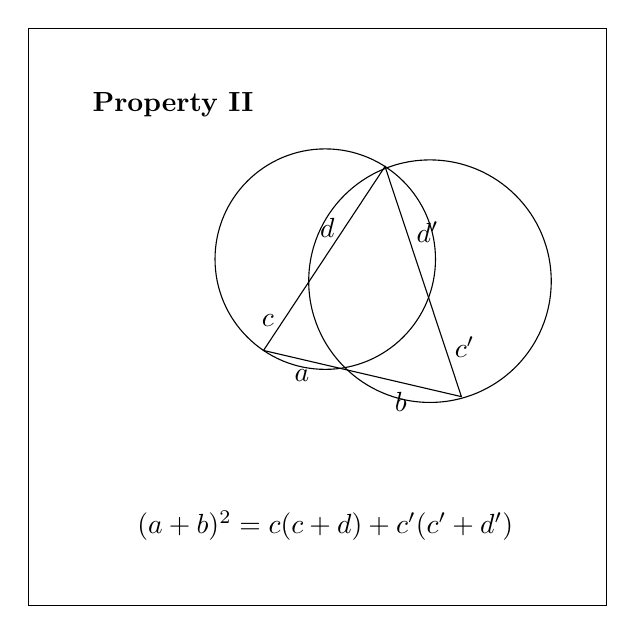
\begin{tikzpicture}[scale=1.4]
    \coordinate (A) at (0.54227, 0.84021);
    \coordinate (B) at (-0.19715, -0.27918);
    \coordinate (C) at (0.93715, -0.34893);
    \coordinate (D) at (0.13538, -0.99079);
    \coordinate (E) at (1.23556, -1.24757);
    \coordinate (F) at (-0.56, -0.82849);
    
    \draw[fill=none] (0,0) circle (1.0);
    \draw[fill=none] (0.95,-0.2) circle (1.1);
    
    \draw (A) -- (F) -- (E) -- cycle;

    \node[left] at ($(A)!0.5!(B)$) {$d$};
    \node[left] at ($(B)!0.5!(F)$) {$c$};
    \node[right] at ($(A)!0.5!(C)$) {$d'$};
    \node[right] at ($(C)!0.5!(E)$) {$c'$};
    \node[below] at ($(F)!0.5!(D)$) {$a$};
    \node[below] at ($(D)!0.5!(E)$) {$b$};

    \node[anchor=north west] at (-2.2, 1.6)
        {\textbf{Property II}};
    \node[anchor=north] at (0, -2.2)
        {$(a+b)^2=c(c+d)+c'(c'+d')$};

    \coordinate (SW) at (current bounding box.south west);
    \coordinate (NE) at (current bounding box.north east);
    \path[draw=black] 
    ($(SW)+(-0.5,-0.5)$) rectangle ($(NE)+(0.5,0.5)$);
\end{tikzpicture}

The properties above may be utilized when the segments
$AB$ and $AC$ are extended because $\square{ABDH}$ and
$\square{AGDC}$ are cyclic.
\begin{center}
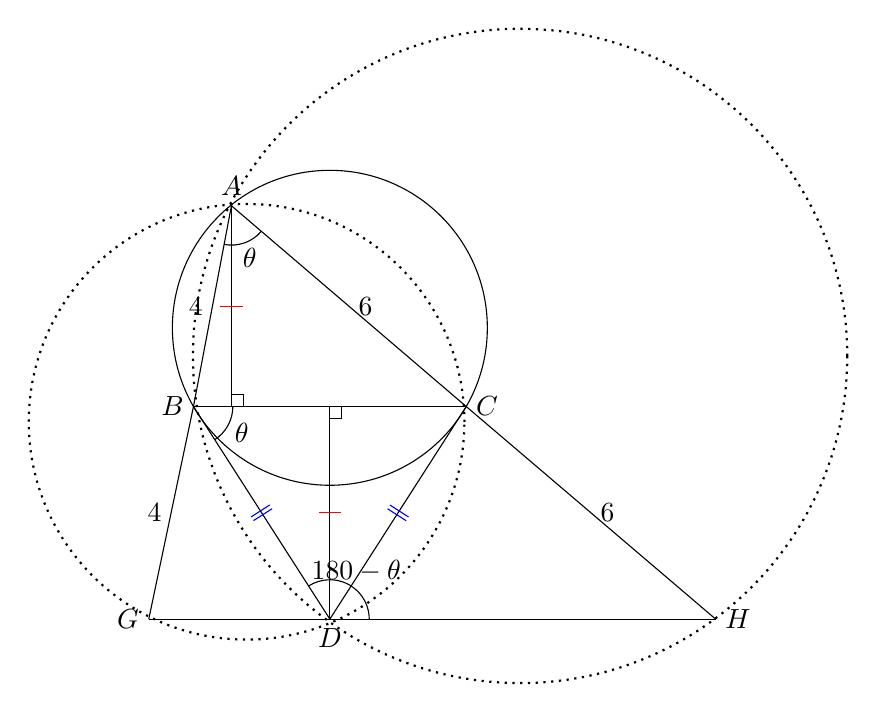
\begin{tikzpicture}
    \coordinate (A) at (-1.25, 1.55);
    \coordinate (B) at (-1.732, -1);
    \coordinate (C) at (1.732, -1);
    \coordinate (D) at (0, -3.7);
    \coordinate (E) at ($(B)!0.5!(C)$);
    \coordinate (F) at (-1.25,-1);
    \coordinate (G) at (-2.3,-3.7);
    \coordinate (H) at (4.9,-3.7);

    \draw (-1.25, -0.85) -- (-1.10, -0.85) -- (-1.10, -1);
    \draw (0, -1.15) -- (0.15, -1.15) -- (0.15, -1);
    
    \draw[fill=none] (0,0) circle (2.0);
    \draw (B) -- (D);
    \draw (C) -- (D);
    \draw (A) -- (F);
    \draw (D) -- (E);
    \draw (B) -- (G);
    \draw (C) -- (H);
    \draw (G) -- (H);
    
    \draw (A) -- (B);
    \draw (B) -- (C);
    \draw (C) -- (A);

    \node[left, above] at (A) {$A$};
    \node[left] at (B) {$B$};
    \node[right] at (C) {$C$};
    \node[below] at (D) {$D$};
    \node[left] at ($(A)!0.5!(B)$) {$4$};
    \node[left] at ($(B)!0.5!(G)$) {$4$};
    \node[right] at ($(A)!0.5!(C)$) {$6$};
    \node[right] at ($(C)!0.5!(H)$) {$6$};
    \node[left] at (G) {$G$};
    \node[right] at (H) {$H$};

    \tkzMarkSegment[color=blue, pos=.5, mark=||](B, D);
    \tkzMarkSegment[color=blue, pos=.5, mark=||](D, C);
    \tkzMarkSegment[color=red, pos=.5, mark=|](A, F);
    \tkzMarkSegment[color=red, pos=.5, mark=|](D, E);

    \draw pic[draw=black, radius=0.1cm, "$\theta$",
        angle eccentricity=1.4] {angle=B--A--C};
    \draw pic[draw=black, radius=0.1cm, "$\theta$",
        angle eccentricity=1.4] {angle=D--B--C};
    \draw pic[draw=black, radius=0.05cm, "$180-\theta$",
        angle eccentricity=1.4] {angle=H--D--B};

    \draw[dotted, thick] (2.41611, -0.357513) circle (4.15483);
    \draw[dotted, thick] (-1.05748, -1.19392) circle (2.76622);
\end{tikzpicture}
\end{center}
Using property of similar triangle and Property II,
\[
(2BC)^2 = 4(4 + 4) + 6(6 + 6) = 104
\]
is true. In another words, $\boxed{BC = \sqrt{26}}$.

\newpage
\section*{Problem}
Let $\triangle{ABC}$, be an acute-angled triangle
with incircle $\omega$ which is tangent to sides
$BC$ and $CA$ at $D$ and $E$, respectively. $X$ is
a point on the altitude from $A$ to $BC$, and the
circle $\omega'$ with diameter $AX$ is tangent to
$\omega$. Denote by $U$ and $V$, respectively, the
points where $CA$ and $AB$ intersect $\omega'$ again.
If $UV = 12$, $AX = 15$ and $AE = 24$, find the value
of $BD \times DC$.

\begin{solution}

\textbf{Key Properties}

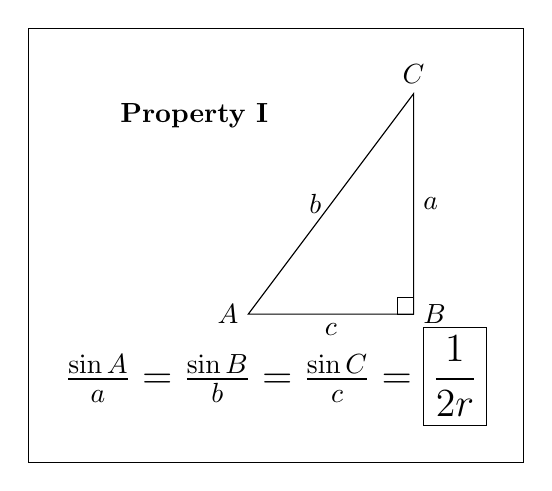
\begin{tikzpicture}[scale=0.7]
    \coordinate (A) at (0, 0);
    \coordinate (B) at (3, 0);
    \coordinate (C) at (3, 4);
    
    \draw (A) -- (B) -- (C) -- cycle;

    \node[below] at ($(A)!0.5!(B)$) {$c$};
    \node[right] at ($(B)!0.5!(C)$) {$a$};
    \node[left] at ($(C)!0.5!(A)$) {$b$};
    \node[left] at (A) {$A$};
    \node[right] at (B) {$B$};
    \node[above] at (C) {$C$};

    \tkzMarkRightAngle[size=.3](A,B,C);

    \node[anchor=north west] at (-2.5,4)
        {\textbf{Property I}};
    \node[anchor=south] at (0.5, -2.2)
        {\Large{$\frac{\sin{A}}{a} = \frac{\sin{B}}{b}
        = \frac{\sin{C}}{c} = \boxed{\frac{1}{2r}}$}};

    \coordinate (SW) at (current bounding box.south west);
    \coordinate (NE) at (current bounding box.north east);
    \path[draw=black] 
    ($(SW)+(-0.5,-0.5)$) rectangle ($(NE)+(0.5,0.5)$);
\end{tikzpicture}
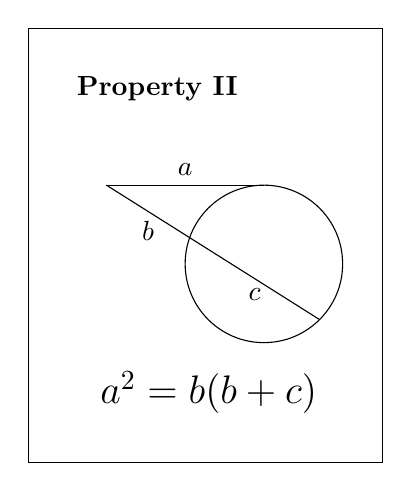
\begin{tikzpicture}
    \coordinate (A) at (-2,1);
    \coordinate (B) at (0,1);
    \coordinate (C) at (0.70710678118,-0.70710678118);
    \coordinate (D) at (-0.94281, 0.33333);

    \draw (0,0) circle (1);

    \draw (A) -- (B);
    \draw (A) -- (C);
    
    \node[above] at ($(A)!0.5!(B)$) {$a$};
    \node[below] at ($(A)!0.5!(D)$) {$b$};
    \node[below] at ($(D)!0.5!(C)$) {$c$};

    \node[anchor=north west] at (-2.5,2.5)
        {\textbf{Property II}};
    \node[anchor=south] at (-0.7, -2.03)
        {\Large{$a^2 = b(b + c)$}};

    \coordinate (SW) at (current bounding box.south west);
    \coordinate (NE) at (current bounding box.north east);
    \path[draw=black] 
    ($(SW)+(-0.5,-0.5)$) rectangle ($(NE)+(0.5,0.5)$);
\end{tikzpicture}
    \\
\tikzset{%
  ->>-/.style={decoration={markings,
               mark=at position 0.5 with {\arrow{>>}}},
               postaction={decorate}},
}
\begin{tikzpicture}[scale=0.741]
    \coordinate (O) at (0, 0);
    \coordinate (O') at (2.5, 2);
    \coordinate (A) at (3.21, 3.64028);
    \coordinate (B) at (1.10593, 0.88143);
    \coordinate (C) at (-0.55752, -1.29968);
    \coordinate (D) at (6.16, 2.36739);
    \coordinate (E) at (-2.34, -0.53134);
    \coordinate (F) at (4.32,-3.40214);
    \coordinate (G) at (0, 5.02535);
    
    
    \draw[fill=none] (O) circle (1.41421356237);
    \draw[fill=none] (O') circle (1.78735279114);
    
    \draw (G) -- (D);
    \draw (E) -- (F);
    
    \draw (O) -- (B);
    \draw (O) -- (C);
    \draw (O') -- (A);
    \draw (O') -- (B);
    \draw (A) -- (C);

    \draw pic[draw=black, "$\theta$",
        angle eccentricity=1.4] {angle=O--B--C};
    \draw pic[draw=black, "$\theta$",
        angle eccentricity=1.4] {angle=O'--B--A};
    \draw pic[draw=black, "$\theta$",
        angle eccentricity=1.4] {angle=B--C--O};
    \draw pic[draw=black, "$\theta$",
        angle eccentricity=1.4] {angle=B--A--O'};
    \draw pic[draw=black, "$90-\theta$",
        angle eccentricity=1.9] {angle=F--C--B};
    \draw pic[draw=black, "$90-\theta$",
        angle eccentricity=1.9] {angle=G--A--B};

    \tkzMarkRightAngle[size=.3](O',A,D);
    \tkzMarkRightAngle[size=.3](O,C,E);

    \foreach \n in {B}
    \node at (\n)[circle,fill,inner sep=1.5pt]{};

    \node[anchor=north west] at (-3.5, 4.5)
        {\textbf{Property III}};

    \draw[<->,thick,shorten >=-60pt,
        shorten <=-60pt,->>-] (G) -- (D);
    \draw[<->,thick,shorten >=-60pt,
        shorten <=-60pt,->>-] (E) -- (F);

    \coordinate (SW) at (current bounding box.south west);
    \coordinate (NE) at (current bounding box.north east);
    \path[draw=black] 
    ($(SW)+(-0.5,-0.5)$) rectangle ($(NE)+(0.5,0.5)$);
\end{tikzpicture}
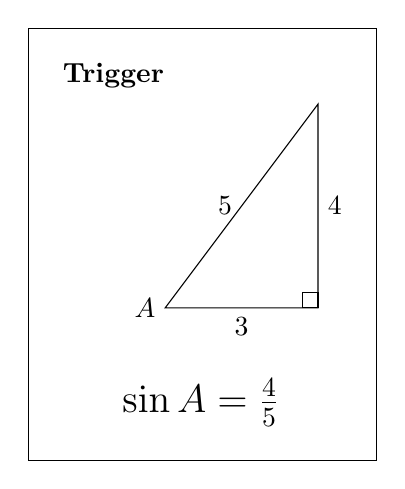
\begin{tikzpicture}[scale=0.647]
    \coordinate (A) at (0, 0);
    \coordinate (B) at (3, 0);
    \coordinate (C) at (3, 4);
    
    \draw (A) -- (B) -- (C) -- cycle;

    \node[below] at ($(A)!0.5!(B)$) {$3$};
    \node[right] at ($(B)!0.5!(C)$) {$4$};
    \node[left] at ($(C)!0.5!(A)$) {$5$};
    \node[left] at (A) {$A$};

    \tkzMarkRightAngle[size=.3](A,B,C);

    \node[anchor=north west] at (-2.2, 5)
        {\textbf{Trigger}};
    \node[anchor=north] at (0.7,-1.2)
        {\Large$\sin{A} = \frac{4}{5}$};

    \coordinate (SW) at (current bounding box.south west);
    \coordinate (NE) at (current bounding box.north east);
    \path[draw=black] 
    ($(SW)+(-0.5,-0.5)$) rectangle ($(NE)+(0.5,0.5)$);
\end{tikzpicture}

\begin{center}
    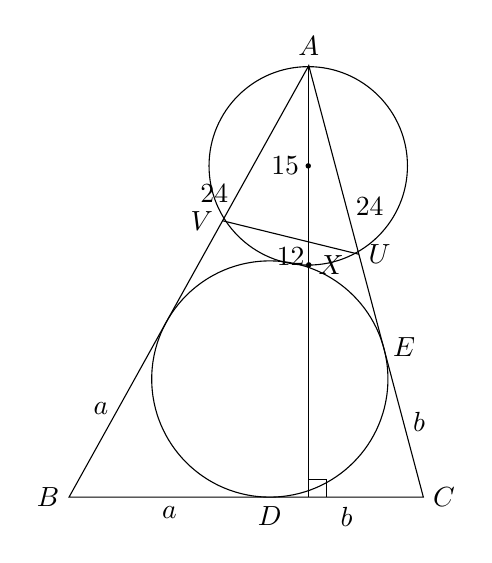
\begin{tikzpicture}[scale=1.5]
        \coordinate (A) at (0.32983, 2.65391);
        \coordinate (B) at (-1.7, -1);
        \coordinate (C) at (1.3, -1);
        \coordinate (D) at (0, -1);
        \coordinate (E) at (0.9618, 0.27375);
        \coordinate (U) at (0.754, 1.05638);
        \coordinate (V) at (-0.4, 1.34013);
        \coordinate (X) at (0.32983, 0.9666);
        \coordinate (F) at (0.32983, -1);
        \coordinate (G) at (-0.871, 0.49228);
        \coordinate (O) at (0.325316, 1.80465);

        \draw (A) -- (B) -- (C) -- cycle;
        \draw[fill=none] (0,0) circle (1);
        \draw[fill=none] (0.325316, 1.80465) circle (0.84);
        \draw (A) -- (F);
        \draw (V) -- (U);

        \node[above] at (A) {$A$};
        \node[left] at (B) {$B$};
        \node[right] at (C) {$C$};
        \node[below] at (D) {$D$};
        \node[right] at (E) {$E$};
        \node[below, right] at (U) {$U$};
        \node[above, left] at (V) {$V$};
        \node[right] at (X) {$X$};

        \node[right] at ($(A)!0.5!(E)$) {$24$};
        \node[right] at ($(E)!0.5!(C)$) {$b$};
        \node[below] at ($(C)!0.5!(D)$) {$b$};
        \node[below] at ($(D)!0.5!(B)$) {$a$};
        \node[left] at ($(B)!0.5!(G)$) {$a$};
        \node[left] at ($(G)!0.5!(A)$) {$24$};
        \node[below] at ($(V)!0.5!(U)$) {$12$};
        \node[left] at ($(A)!0.5!(X)$) {$15$};
        
        \draw (0.32983, -0.85) -- (0.47983, -0.85)
            -- (0.47983, -1);

        \foreach \n in {O, X}
        \node at (\n)[circle,fill,inner sep=0.7pt]{};
    \end{tikzpicture}
\end{center}
The properties may be utilized to further modify
the diagram.
\begin{center}
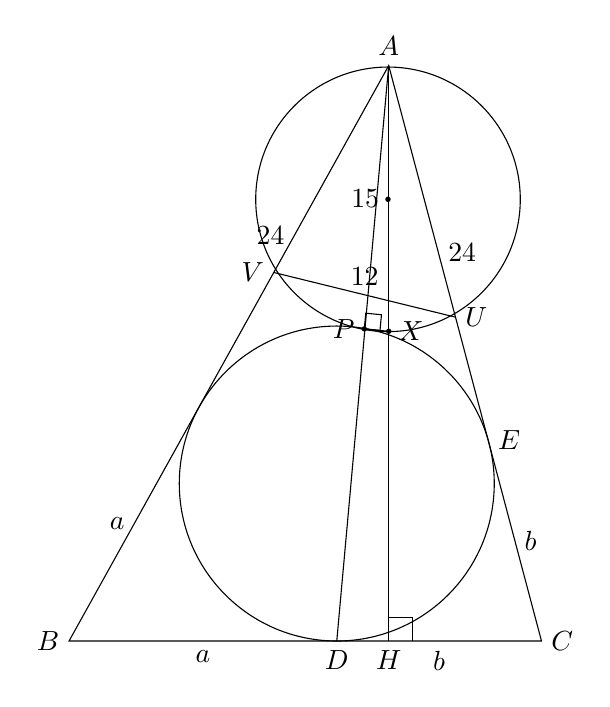
\begin{tikzpicture}[scale=2]
    \coordinate (A) at (0.32983, 2.65391);
    \coordinate (B) at (-1.7, -1);
    \coordinate (C) at (1.3, -1);
    \coordinate (D) at (0, -1);
    \coordinate (E) at (0.9618, 0.27375);
    \coordinate (U) at (0.754, 1.05638);
    \coordinate (V) at (-0.4, 1.34013);
    \coordinate (X) at (0.32983, 0.9666);
    \coordinate (F) at (0.32983, -1);
    \coordinate (G) at (-0.871, 0.49228);
    \coordinate (O) at (0.325316, 1.80465);
    \coordinate (P) at (0.175,0.982);
    \coordinate (H) at (0.32983, -1);

    \draw (A) -- (B) -- (C) -- cycle;
    \draw[fill=none] (0,0) circle (1);
    \draw[fill=none] (0.325316, 1.80465) circle (0.84);
    \draw (A) -- (F);
    \draw (V) -- (U);
    \draw (A) -- (D);
    \draw (P) -- (X);

    \node[above] at (A) {$A$};
    \node[left] at (B) {$B$};
    \node[right] at (C) {$C$};
    \node[below] at (D) {$D$};
    \node[right] at (E) {$E$};
    \node[below, right] at (U) {$U$};
    \node[above, left] at (V) {$V$};
    \node[right] at (X) {$X$};
    \node[left] at (P) {$P$};
    \node[below] at (H) {$H$};

    \node[right] at ($(A)!0.5!(E)$) {$24$};
    \node[right] at ($(E)!0.5!(C)$) {$b$};
    \node[below] at ($(C)!0.5!(D)$) {$b$};
    \node[below] at ($(D)!0.5!(B)$) {$a$};
    \node[left] at ($(B)!0.5!(G)$) {$a$};
    \node[left] at ($(G)!0.5!(A)$) {$24$};
    \node[above] at ($(V)!0.5!(U)$) {$12$};
    \node[left] at ($(A)!0.5!(X)$) {$15$};

    \tkzMarkRightAngle[size=.1](A,P,X);
    
    \draw (0.32983, -0.85) -- (0.47983, -0.85)
        -- (0.47983, -1);

    \foreach \n in {O, X, P}
    \node at (\n)[circle,fill,inner sep=0.7pt]{};
\end{tikzpicture}
\end{center}
Using the property of similar triangle, it is
evident that $\frac{AP}{AX} = \frac{AH}{AD}$.
Using Power of a Point theorem, $AH = \frac{24^2}{15}$.
Because $AH$ is known, an impulse to use area formulas is
created. Heron's Formula, area formula using the radius of
inscribed circle, and the fundamental formula are the
possible options.

From Property I, $\frac{\sin{A}}{12} = \frac{1}{15}$.
In another words, $\sin{A} = \frac{4}{5}$.
\begin{center}
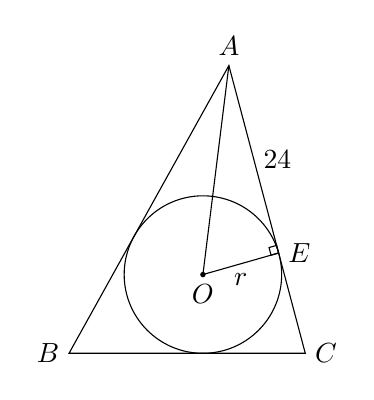
\begin{tikzpicture}
    \coordinate (A) at (0.32983, 2.65391);
    \coordinate (B) at (-1.7, -1);
    \coordinate (C) at (1.3, -1);
    \coordinate (E) at (0.9618, 0.27375);
    \coordinate (O') at (0,0);

    \draw (A) -- (B) -- (C) -- cycle;
    \draw[fill=none] (0,0) circle (1);
    \draw (O') -- (E);
    \draw (A) -- (O');

    \node[above] at (A) {$A$};
    \node[left] at (B) {$B$};
    \node[right] at (C) {$C$};
    \node[right] at (E) {$E$};
    \node[left, below] at (O') {$O$};
    \node[below] at ($(O')!0.5!(E)$) {$r$};

    \node[right] at ($(A)!0.5!(E)$) {$24$};

    \tkzMarkRightAngle[size=.1](O',E,A);
    
    \node at (O')[circle,fill,inner sep=0.7pt]{};
\end{tikzpicture}
\end{center}
From the extracted diagram, a new diagram may be form.
\begin{center}
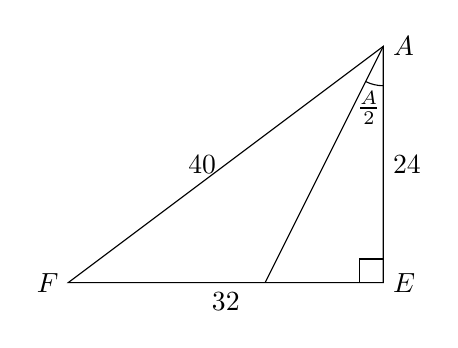
\begin{tikzpicture}
    \coordinate (A) at (0, 0);
    \coordinate (B) at (4, 0);
    \coordinate (C) at (4, 3);
    \coordinate (D) at (2.5,0);
    
    \draw (A) -- (B) -- (C) -- cycle;
    \draw (C) -- (D);

    \node[below] at ($(A)!0.5!(B)$) {$32$};
    \node[above, right] at ($(B)!0.5!(C)$) {$24$};
    \node[left] at ($(C)!0.5!(A)$) {$40$};
    \node[above, right] at (C) {$A$};
    \node[right] at (B) {$E$};
    \node[left] at (A) {$F$};

    \tkzMarkRightAngle[size=.3](A,B,C);
    \draw pic[draw=black, "$\frac{A}{2}$",
        angle eccentricity=1.6] {angle=D--C--B};
\end{tikzpicture}
\end{center}
The Angle Bisector Theorem manifests that
$r = 32 \cdot \frac{24}{40 + 24} = 12$.

The area formula involving the radius of inscribed
circle and the fundamental formula provides the
following equation.
\begin{align*}
    \frac{1}{2} \cdot 12 \cdot (2a + 2b + 48)
    &= \frac{1}{2} \cdot \frac{24^2}{15} \cdot (a + b) \\
    (2a + 2b + 48) &= \frac{48}{15} \cdot (a + b) \\
    (2a + 2b + 48) &= \frac{16}{5} \cdot (a + b) \\
    10(a + b) + 240 &= 16(a + b) \\
    a + b &= 40 \\
\end{align*}
The area could be represented in different form
using the Heron's Formula.
\begin{align*}
    \text{Let } S=
    &\frac{24 + a + 24 + b + a + b}{2} = a + b + 24 \\
    \text{Area}
    &= \sqrt{S(S - 24 - a)(S - 24 - b)(S - a - b)} \\
    &= \sqrt{24ab (a + b + 24)}
\end{align*}
\[
\frac{1}{2} \cdot 12 \cdot (2a + 2b + 48)
= \sqrt{24ab (a + b + 24)}
\]
is true.
\begin{align*}
    \frac{1}{2} \cdot 12 \cdot (2a + 2b + 48)
    &= \sqrt{24ab(a + b + 24)} \\
    6 (128) &= \sqrt{24ab (64)} \\
    6 (128) &= 16 \sqrt{6ab} \\
    24 &= \sqrt{6ab} \\
    ab &= 96 \\
\end{align*}
Therefore, $\boxed{BD \cdot DC = 96}$.
\end{solution}

\end{document}


